\documentclass[11pt]{article}

\usepackage{amsmath}
\usepackage{amssymb}
\usepackage[margin=0.68in]{geometry}
\usepackage{booktabs}
\usepackage{enumitem}
\usepackage{fancyhdr}
\usepackage{graphicx}
\usepackage[table]{xcolor}
\usepackage[hidelinks]{hyperref}
\usepackage{listings}
\usepackage{microtype}
\usepackage{tabularx}
\usepackage{tikz}
\usepackage{titlesec}
\usetikzlibrary{arrows.meta,decorations.pathmorphing,positioning,shapes.geometric}
\graphicspath{{docs/lessons/assets/}{../assets/}}

\definecolor{Ink}{gray}{0}
\definecolor{CodeGray}{gray}{0.96}
\definecolor{Soft}{gray}{0.90}
\hypersetup
{
    pdftitle={ADK Lesson 024: Observable Greenhouse Trainer},
    pdfauthor={Kevin Shanahan},
    pdfsubject={Deterministic moisture, bounded watering intent, presentation, and stable records},
    pdflang={en-US}
}
\pagestyle{fancy}
\fancyhf{}
\lhead{\textsc{ADK Lesson 024}}
\rhead{Observable Greenhouse Trainer}
\cfoot{\thepage}
\setlength{\headheight}{14pt}
\setlength{\parindent}{0pt}
\setlength{\parskip}{5pt}
\setlist{nosep,leftmargin=1.45em}
\titleformat{\section}{\Large\bfseries\color{Ink}}{\thesection}{0.5em}{}
\titleformat{\subsection}{\large\bfseries\color{Ink}}{\thesubsection}{0.5em}{}
\lstdefinestyle{adkcpp}
{
    language=C++,
    backgroundcolor=\color{CodeGray},
    basicstyle=\ttfamily\small,
    keywordstyle=\color{Ink}\bfseries,
    commentstyle=\color{Ink},
    columns=fullflexible,
    keepspaces=true,
    showstringspaces=false,
    frame=single,
    rulecolor=\color{Ink},
    breaklines=true,
    tabsize=4
}
\newcommand{\lessonbox}[1]{%
  \begin{center}
  \fcolorbox{Ink}{white}{\parbox{0.92\linewidth}{#1}}
  \end{center}}

\begin{document}

\begin{center}
  {\Huge\bfseries Observable Greenhouse Trainer}\\[4pt]
  {\Large Observe, decide, actuate, present, record}\\[8pt]
  \textit{A deterministic project with visible evidence and no energetic load}
\end{center}

\begin{tabularx}{\linewidth}{@{}>{\bfseries}l X >{\bfseries}l X@{}}
Lesson & 024 --- project & Time & 45--75 minutes\\
Prerequisites & Lessons 001--023 & Board & Arduino Mega 2560\\
Evidence & TP-M, D38, D13, RGB, LCD & Status & host verified\\
Energy class & E1: USB, passive input, LCD, and resistor-limited LEDs only\\
\end{tabularx}

\lessonbox{\textbf{Hard boundary.} ``Pump'' means the LED on D38. Do not
connect a relay, motor, pump, heater, water, external load supply, or mains
circuit. The fixed storage medium is an in-memory teaching model, not an SD
card. ADK is not an unattended irrigation or safety controller.}

\section{Mission and dependency map}

Build one replayable chain. TP-M feeds \texttt{MoistureSensor}; its sample
reaches \texttt{WateringController}, then \texttt{PanelPumpOutput}, then
\texttt{InertLoadPanel}. The same decided state also feeds the LCD view, stable
record, and RGB mode evidence.

\begin{center}
% ADK visual: pencil
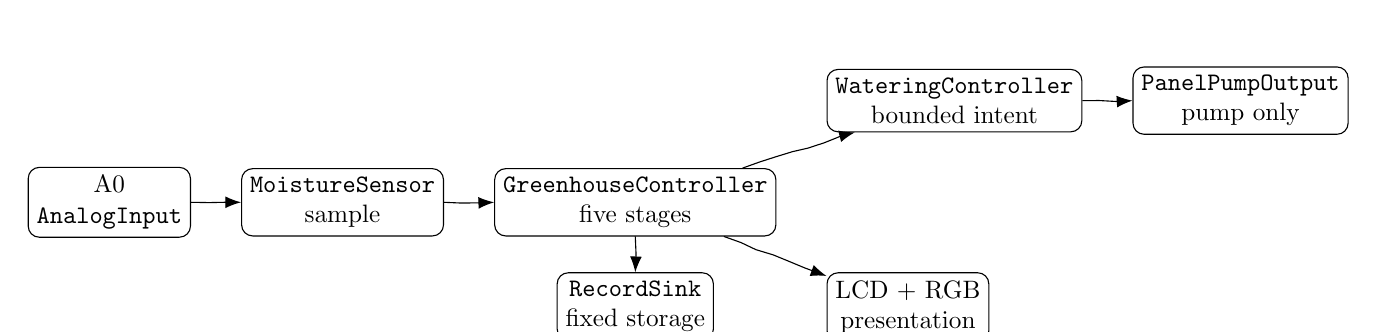
\begin{tikzpicture}[scale=0.91,transform shape,
  node distance=5mm and 7mm,
  box/.style={draw,rounded corners,align=center,minimum height=8mm},
  pencil/.style={-{Latex[length=2mm]},decorate,
    decoration={random steps,segment length=2.2mm,amplitude=.12mm}}
]
  \node[box] (input) {A0\\\texttt{AnalogInput}};
  \node[box,right=of input] (moisture) {\texttt{MoistureSensor}\\sample};
  \node[box,right=of moisture] (greenhouse) {\texttt{GreenhouseController}\\five stages};
  \node[box,above right=of greenhouse] (watering) {\texttt{WateringController}\\bounded intent};
  \node[box,right=of watering] (pump) {\texttt{PanelPumpOutput}\\pump only};
  \node[box,below right=of greenhouse] (view) {LCD + RGB\\presentation};
  \node[box,below=of greenhouse] (record) {\texttt{RecordSink}\\fixed storage};
  \draw[pencil] (input) -- (moisture);
  \draw[pencil] (moisture) -- (greenhouse);
  \draw[pencil] (greenhouse) -- (watering);
  \draw[pencil] (watering) -- (pump);
  \draw[pencil] (greenhouse) -- (view);
  \draw[pencil] (greenhouse) -- (record);
\end{tikzpicture}
\end{center}

The arrows are ownership or explicit borrowing relationships, not hidden
global access. The coordinator owns dependency lifecycle calls; caller-owned
objects outlive it.

\section{Orientation and exact circuit}

\begin{center}
% ADK visual: pencil
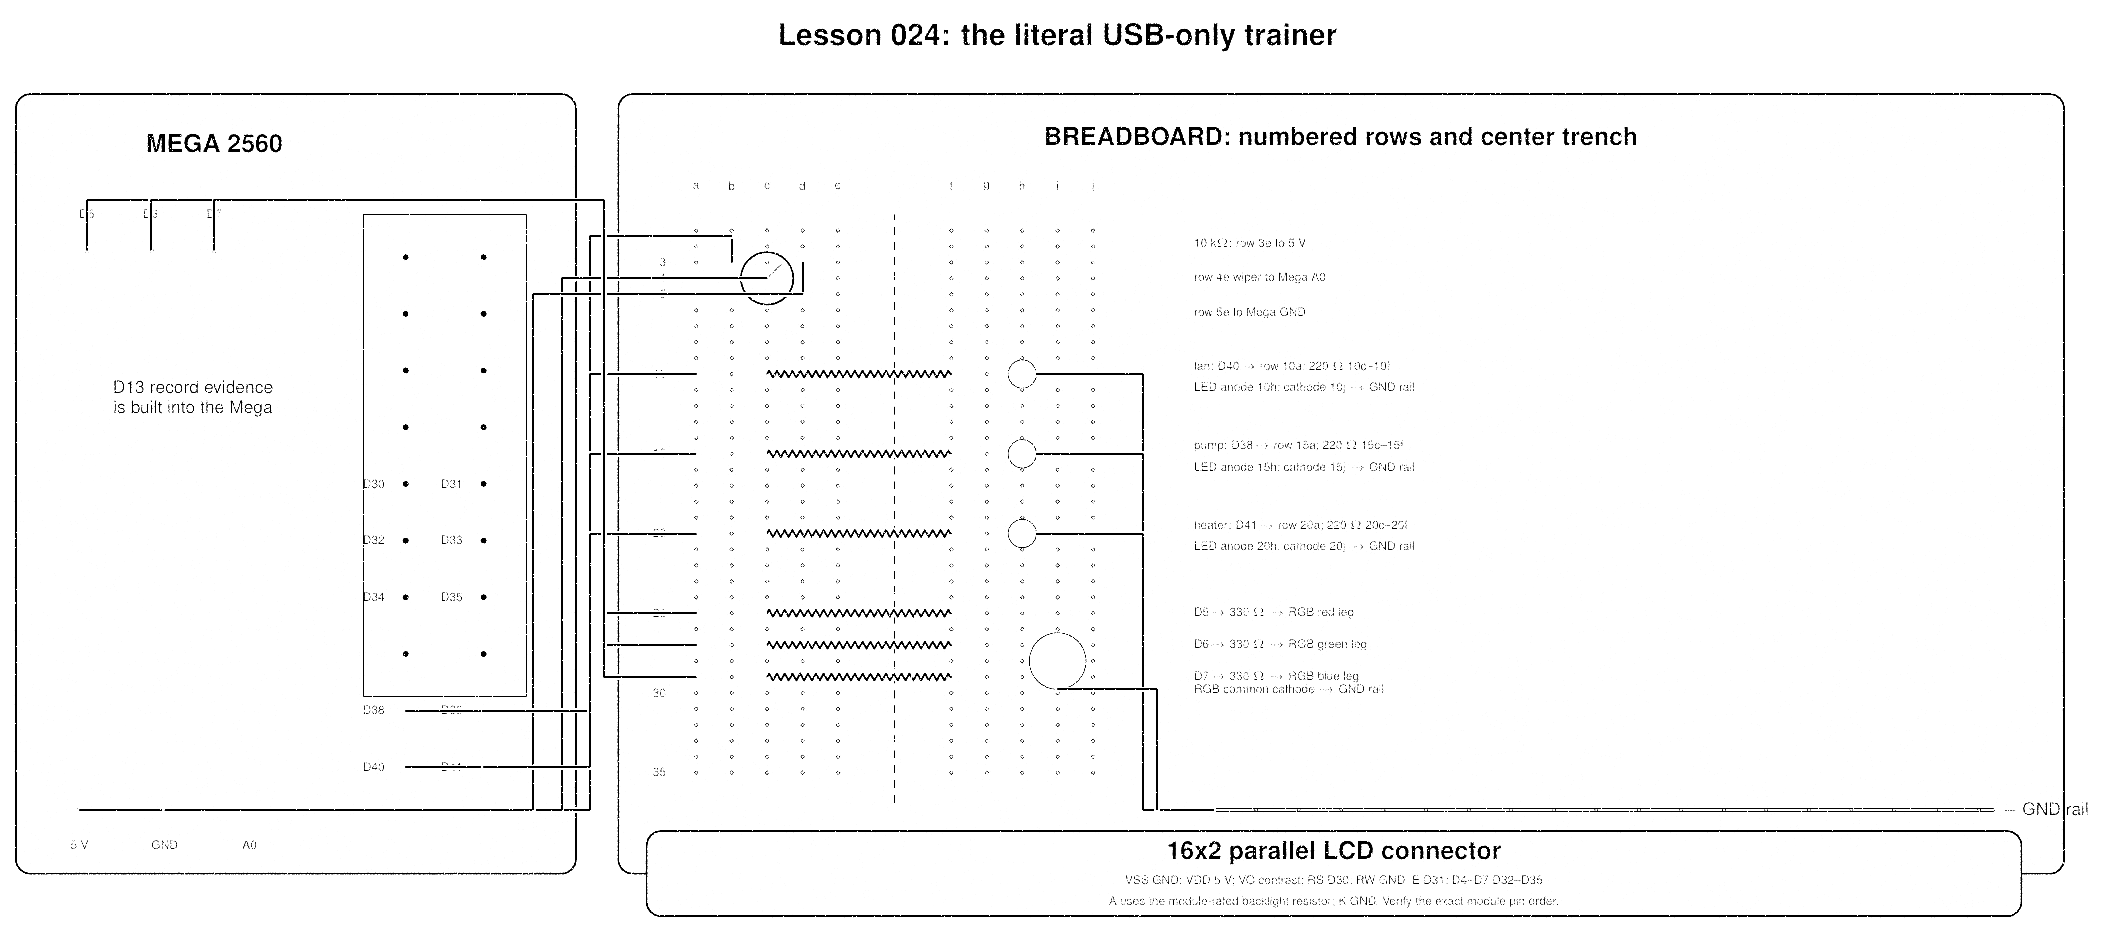
\includegraphics[width=0.94\linewidth]{024-greenhouse-pencil.png}
\end{center}
\textit{Alternative text: literal Mega and numbered-breadboard plate. It shows
the paired D30--D41 header, top-header D5--D7, A0, 5 V, and GND; exact
potentiometer rows; three separate resistor--LED--ground paths; three RGB
series paths; and the parallel LCD connector. D13 is explicitly the built-in
LED. The plate contains no relay or external load.}

\begin{center}
% ADK visual: pencil
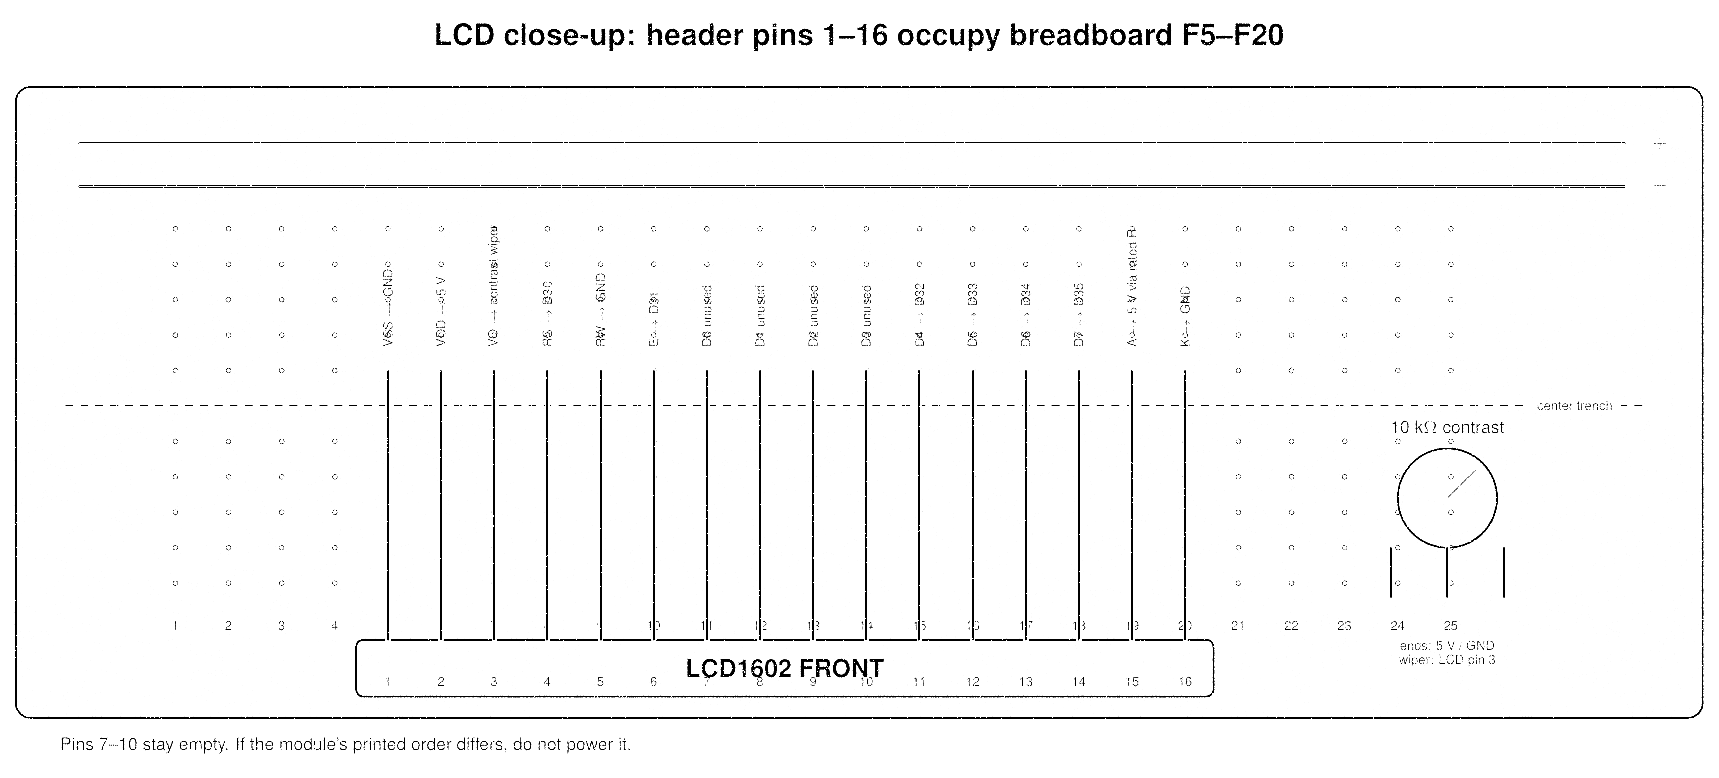
\includegraphics[width=0.98\linewidth]{024-lcd-closeup.png}
\end{center}
\textit{Alternative text: close-up of all sixteen LCD header positions,
numbered 1 through 16 in breadboard holes F5 through F20. Every used supply,
contrast, control, four-bit data, and backlight connection is labeled; D0
through D3 remain empty.}

The drawing helps locate parts; this table is authoritative.

\begin{tabularx}{\linewidth}{@{}l l X@{}}
\toprule
Meaning & Pin & Connection\\
\midrule
Moisture simulator / TP-M & A0 / D54 & 10 k\(\Omega\) potentiometer wiper\\
Potentiometer ends & 5 V, GND & one end to each USB-powered rail\\
Simulated fan & D40 & 220 \(\Omega\), LED anode; cathode to GND\\
Simulated pump / TP38 & D38 & 220 \(\Omega\), LED anode; cathode to GND\\
Simulated heater & D41 & 220 \(\Omega\), LED anode; cathode to GND\\
Record acknowledgement & D13 & built-in LED\\
Mode evidence & D5, D6, D7 & RGB channels, one 330 \(\Omega\) resistor each\\
LCD control/data & D30--D35 & RS, E, D4, D5, D6, D7\\
LCD supply & 5 V, GND & exact module rating and contrast network\\
\bottomrule
\end{tabularx}

\textbf{Before USB:} trace each signal from its labeled Mega pin, through one
series resistor and LED, to GND. Check the LCD's printed pin order against the
table. If the module differs, stop at the three-LED build and leave the LCD
unplugged. There is no relay or external supply in this lesson.

\section{Four quick wins}

\begin{center}
% ADK visual: pencil
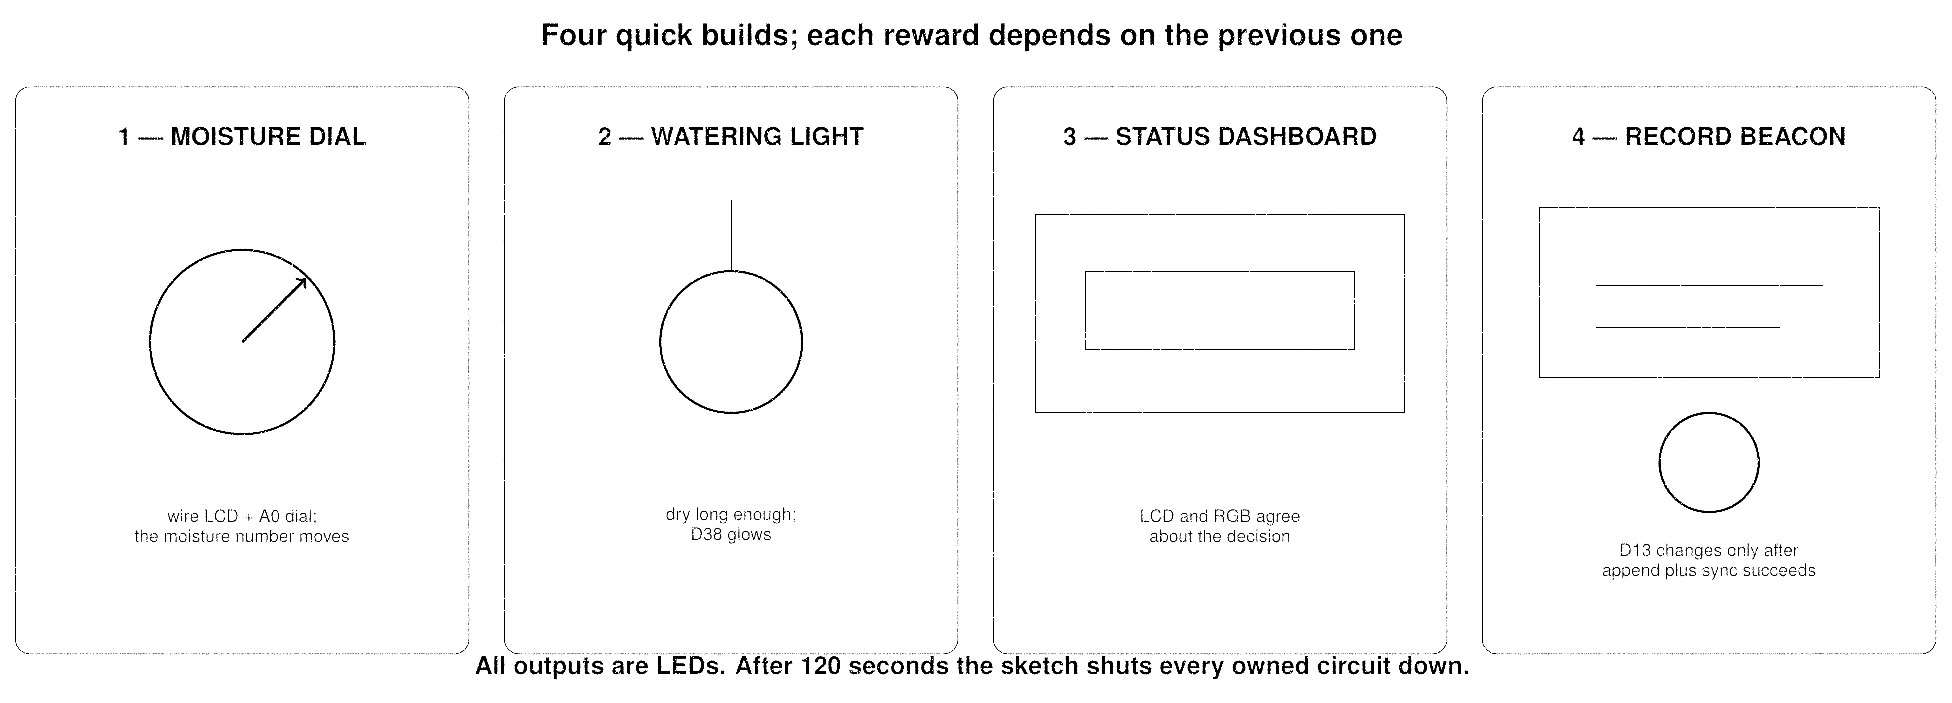
\includegraphics[width=0.98\linewidth]{024-greenhouse-progress.png}
\end{center}
\textit{Alternative text: four panels show the dependent progression:
potentiometer-controlled moisture number, dry-triggered D38 watering LED,
LCD-and-RGB status dashboard, and D13 acknowledgement after an in-memory
record append and sync.}

\begin{enumerate}
  \item Wire the potentiometer and LCD. Turning the dial must move the moisture
        value; if it does not, later stages cannot make a valid decision.
  \item Add D38 and its resistor. Hold the dial in the dry region: after the
        minimum-off interval D38 lights. Turn wet and it goes dark.
  \item Add the RGB channels. Their pattern and the LCD words must explain the
        same D38 decision. Every eight seconds inhibition creates an amber,
        D38-dark intermission without another input part.
  \item Watch built-in D13. It changes only after a complete record is appended
        and synchronized in the fixed RAM model.
\end{enumerate}

At 120 seconds the sketch shuts down the controller and every owned evidence
output. Press Reset for another run.

\section{The narrative loop}

\begin{lstlisting}[style=adkcpp]
const adk::TimePoint now (millis ());

observeGreenhouse (now);
decideGreenhouse  (now);
actuateGreenhouse (now);
presentGreenhouse (now);
recordGreenhouse  (now);
showGreenhouseHealth(now);
\end{lstlisting}

\texttt{observe()} samples at most once when due. \texttt{decide()} changes
policy and intent but no output. \texttt{actuate()} is the only stage allowed
to change D38. \texttt{present()} writes an already-decided LCD view.
\texttt{record()} publishes the same decision. Missed periods coalesce; they do
not create a burst.

\section{Watering policy and state graph}

The reference calibration maps raw 800 to dry (0 permille) and raw 200 to wet
(1000 permille). Watering may begin below 350 only after 2000 ms off. It stops
at or above 600, on inhibition, on invalid or stale sensing, or after 5000 ms
on. Maximum-on creates a lockout; another dry sample cannot clear it early.
\texttt{PanelPumpOutput} maps on to the panel's pump channel and off to none.
The fan and heater indicators remain off throughout this project.

\begin{center}
% ADK visual: pencil
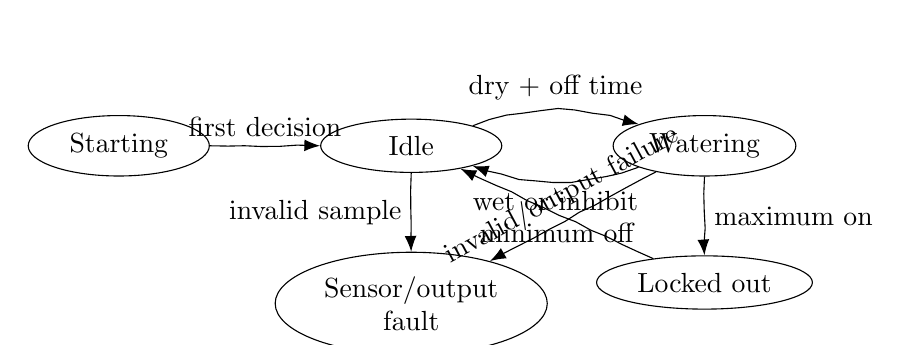
\begin{tikzpicture}[
  node distance=10mm and 14mm,
  state/.style={draw,ellipse,align=center,minimum width=23mm},
  pencil/.style={-{Latex[length=2mm]},decorate,
    decoration={random steps,segment length=2.2mm,amplitude=.12mm}}
]
  \node[state] (start) {Starting};
  \node[state,right=of start] (idle) {Idle};
  \node[state,right=of idle] (water) {Watering};
  \node[state,below=of water] (lock) {Locked out};
  \node[state,below=of idle] (fault) {Sensor/output\\fault};
  \draw[pencil] (start) -- node[above]{first decision} (idle);
  \draw[pencil,bend left=18] (idle) to node[above]{dry + off time} (water);
  \draw[pencil,bend left=18] (water) to node[below]{wet or inhibit} (idle);
  \draw[pencil] (water) -- node[right]{maximum on} (lock);
  \draw[pencil] (lock) -- node[below]{minimum off} (idle);
  \draw[pencil] (idle) -- node[left]{invalid sample} (fault);
  \draw[pencil] (water) -- node[above,sloped]{invalid/output failure} (fault);
\end{tikzpicture}
\end{center}

\begin{tabularx}{\linewidth}{@{}l X l@{}}
\toprule
Condition & Decision & D38\\
\midrule
Invalid, unavailable, or stale sample & sensor fault dominates & off\\
Operator inhibition & intent forced off & off\\
On-time at or beyond maximum & lockout & off\\
Valid sample at or above wet threshold & stop watering & off\\
Valid sample below dry threshold after off-time & begin watering & on\\
Between thresholds & preserve safe current state & unchanged\\
\bottomrule
\end{tabularx}

\section{Mode precedence and independent evidence}

\begin{tabularx}{\linewidth}{@{}l X X@{}}
\toprule
Mode & RGB pattern & Narrow interpretation\\
\midrule
Starting & slow blue pulse & lifecycle/schedule start\\
Monitoring & green heartbeat & valid sample; pump intent off\\
Watering & cyan heartbeat & D38 requested on\\
Inhibited & steady amber & software policy denied watering\\
SensorFault & two red pulses & sample unusable\\
OutputFault & steady red & command failure latched\\
DisplayFault & three amber pulses & LCD cannot report itself\\
RecordFault & four red pulses & append or sync failed\\
MultipleFaults & steady red & output plus another fault\\
\bottomrule
\end{tabularx}

Output failure dominates and latches until successful reinitialization. Sensor
failure and inhibition always suppress watering. A display or record failure
cannot enable D38.

\subsection{Read the visible story}

\begin{enumerate}
  \item \textbf{Acquisition.} LCD startup and the first RGB transition show
        that the visible system acquired its resources.
  \item \textbf{Safe state.} D38 stays dark at startup, inhibition, invalid
        sensing, and shutdown.
  \item \textbf{Record boundary.} D13 changes only after append and sync
        succeed. It means the RAM model accepted a record, never SD durability.
\end{enumerate}

If a later reward appears without the earlier one, remove USB and retrace that
stage's numbered rows. Serial is not needed to enjoy or diagnose the build.

\section{What the visible sequence means}

\begin{tabularx}{\linewidth}{@{}r r c X X X@{}}
\toprule
ms & raw & allowed & visible result & D38 & record\\
\midrule
0 & 500 & yes & monitoring & off & first accepted\\
1999 & 700 & yes & dry; waiting & off & cadence continues\\
2000 & 700 & yes & watering & on & decision captured\\
4500 & 440 & yes & wet threshold & off & stop captured\\
6500 & 700 & yes & watering may restart & on & decision captured\\
8000 & 700 & no & amber inhibited & off & inhibition captured\\
16000 & 700 & yes & policy resumes & timing decides & cadence continues\\
\bottomrule
\end{tabularx}

The repository's automated tests replay exact timestamp and fault traces
behind the scenes while the learner experience stays with the visible
dependent sequence.

\section{Stable records, storage, and time}

Version 1 uses bounded locale-independent ASCII:

\begin{lstlisting}[style=adkcpp]
adk-gh,1,17,42000,valid,472,340,on,dry,watering
\end{lstlisting}

Fields are format, version, sequence, decision milliseconds, sample state, raw
reading, moisture permille or a dash, requested pump, reason, and mode.
Sequence advances only after successful acceptance. One failed pending record
keeps its original timestamp and bytes during retry.

\texttt{FixedStorage} distinguishes staged bytes from a durable prefix:
\texttt{append()} alone is not durability; \texttt{sync()} advances the durable
prefix. Shutdown and restart discard an unsynchronized suffix. This is an
executable storage model in RAM, not evidence for an SD card.

The public \texttt{Rtc} boundary distinguishes valid, unset,
oscillator-stopped, and transport-fault readings. The deterministic
\texttt{SimulatedRtc} returns a fixed epoch plus a sequence. The record sink
requires a valid reading before append and sync. No physical RTC adapter is
selected, so the record schema still uses explicit \texttt{TimePoint}
milliseconds.

\section{Fault matrix and diagnosis}

\begin{tabularx}{\linewidth}{@{}l X X@{}}
\toprule
Injected condition & Required response & Evidence to retain\\
\midrule
Calibration invalid & initialization rejects, no output claim & complete rollback\\
Range or stale sample & D38 off; sensor fault visible & raw reading and state\\
Output command failure & best-effort off; latched output fault & full status\\
LCD write failure & watering state unchanged & RGB display-fault pattern\\
Append failure & pending record retained & original bytes and sequence\\
Sync failure & no durability claim; retry same record & D13 does not acknowledge\\
Delayed stage call & one coalesced operation & timestamp and next snapshot\\
Shutdown in any mode & dependencies close in reverse & TP38 safe state\\
\bottomrule
\end{tabularx}

\begin{center}
% ADK visual: pencil
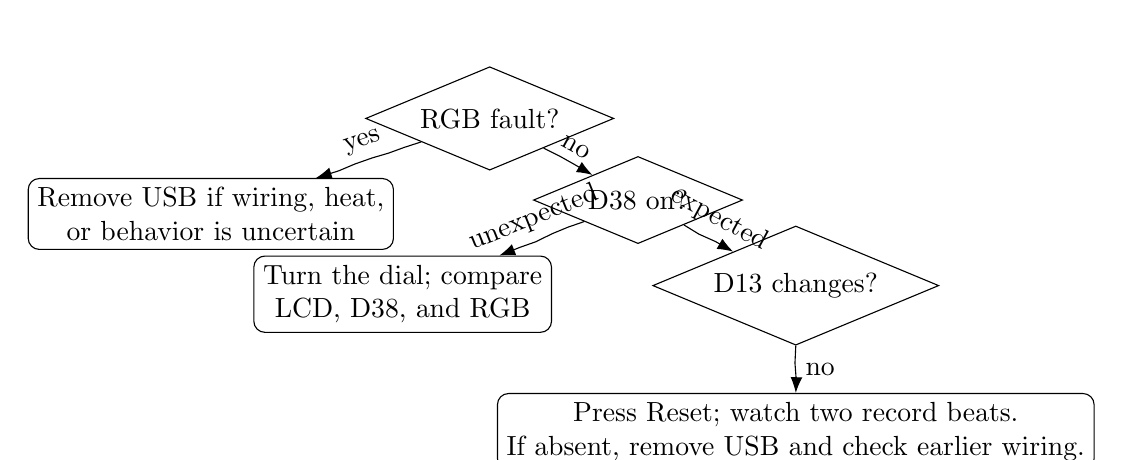
\begin{tikzpicture}[
  node distance=6mm,
  q/.style={draw,diamond,aspect=2.4,align=center},
  a/.style={draw,rounded corners,align=center},
  pencil/.style={-{Latex[length=2mm]},decorate,
    decoration={random steps,segment length=2.2mm,amplitude=.12mm}}
]
  \node[q] (rgb) {RGB fault?};
  \node[a,below left=of rgb] (safe) {Remove USB if wiring, heat,\\or behavior is uncertain};
  \node[q,below right=of rgb] (pump) {D38 on?};
  \node[a,below left=of pump] (sensor) {Turn the dial; compare\\LCD, D38, and RGB};
  \node[q,below right=of pump] (record) {D13 changes?};
  \node[a,below=of record] (host) {Press Reset; watch two record beats.\\If absent, remove USB and check earlier wiring.};
  \draw[pencil] (rgb) -- node[above,sloped]{yes} (safe);
  \draw[pencil] (rgb) -- node[above,sloped]{no} (pump);
  \draw[pencil] (pump) -- node[above,sloped]{unexpected} (sensor);
  \draw[pencil] (pump) -- node[above,sloped]{expected} (record);
  \draw[pencil] (record) -- node[right]{no} (host);
\end{tikzpicture}
\end{center}

Never diagnose by shorting, hot-plugging bare wires, or attaching a real load.

\section{Safe finish and honest claims}

The last reward is the shutdown: at 120 seconds D38, the other inert-load LEDs,
the RGB indicator, display, record sink, moisture input, and their resource
claims all close in dependency-safe order. Remove USB before changing wires.

An LED and fixed-storage model cannot establish pump electrical behavior, SD
durability, RTC accuracy, water delivery, plant health, or unattended safety.
No physical RTC, media adapter, pump, relay, heater, or water path is part of
this build, and no bench verification is claimed by this document.

\section{References and next step}

\begin{itemize}
  \item \href{https://github.com/spincyc/adk/tree/main/examples/Lesson024GreenhouseTrainer}
  {Canonical Lesson 024 sketch}
  \item \href{https://github.com/spincyc/adk/blob/main/src/greenhouse_controller.h}
  {Controller interface} and
  \href{https://github.com/spincyc/adk/blob/main/tests/test_greenhouse_controller.cpp}
  {deterministic tests}
  \item \href{https://github.com/spincyc/adk/blob/main/docs/design/LESSONS_022_024.md}
  {Lessons 022--024 design record} and
  \href{https://github.com/spincyc/adk/blob/main/docs/SAFETY_MODEL.md}
  {ADK safety model}
  \item \href{https://docs.arduino.cc/hardware/mega-2560}
  {Arduino Mega 2560 Rev3 documentation}
  \item \href{https://docs.arduino.cc/learn/programming/sd-guide/}
  {Arduino data-logging guide}
\end{itemize}

The HTML reference carries searchable API links. This PDF is the printable
build adventure. Next, Lesson 025 separates captured infrared timing evidence
from decoded command policy.

\end{document}
